\documentclass{article}

\usepackage{geometry}
\usepackage{amsmath}
\usepackage{graphicx, eso-pic}
\usepackage{listings}
\usepackage{hyperref}
\usepackage{multicol}
\usepackage{fancyhdr}
\pagestyle{fancy}
\fancyhf{}
\hypersetup{ colorlinks=true, linkcolor=black, filecolor=magenta, urlcolor=cyan}
\geometry{ a4paper, total={170mm,257mm}, top=20mm, right=20mm, bottom=20mm, left=20mm}
\lhead{Seleksi Tahap 1 Laboratorium Pemrograman 2019}
\setlength{\parindent}{0pt}
\setlength{\parskip}{0.3em}
\renewcommand{\headrulewidth}{0pt}
\rfoot{\thepage}
\lfoot{Seleksi Tahap 1 Labpro 2019}
\lstset{
    basicstyle=\ttfamily\small,
    columns=fixed,
    extendedchars=true,
    breaklines=true,
    tabsize=2,
    prebreak=\raisebox{0ex}[0ex][0ex]{\ensuremath{\hookleftarrow}},
    frame=none,
    showtabs=false,
    showspaces=false,
    showstringspaces=false,
    prebreak={},
    keywordstyle=\color[rgb]{0.627,0.126,0.941},
    commentstyle=\color[rgb]{0.133,0.545,0.133},
    stringstyle=\color[rgb]{01,0,0},
    captionpos=t,
    escapeinside={(\%}{\%)}
}

\begin{document}

\begin{center}
    \section*{Mencari Tempat Perkumpulan} % ganti judul soal

    \begin{tabular}{ | c c | }
        \hline
        Batas Waktu  & 1s \\    % jangan lupa ganti time limit
        Batas Memori & 128MB \\  % jangan lupa ganti memory limit
        \hline
    \end{tabular}
\end{center}

\subsection*{Deskripsi}
Diberikan perumahan dengan N rumah yang merupakan suatu connected graph, dengan setiap simpul berupa rumah dan antar rumah terdapat jalan dengan jarak tertentu. Anda diberikan nomor dari tiga rumah, yakni nomor rumah Nobita, nomor rumah Suneo, dan nomor rumah Giant. Kemudian, didefinisikan nilai $S_i$ sebagai nilai dari:

\begin{center}
    $S_i$ = max(jarak terdekat rumah Nobita ke rumah-$i$,
    jarak terdekat rumah Suneo ke rumah-$i$,
    jarak terdekat rumah Giant ke rumah-$i$)    
\end{center}


Nobita, Suneo, dan Giant ingin kumpul di suatu rumah-$X$ sedemikian sehingga nilai $S_X$ merupakan nilai minimum dari semua $S_i$ yang ada. Tentukan nilai $X$ tersebut (Jika ada lebih dari satu $X$ yang memenuhi, pilih nomor yang lebih kecil)

\subsection*{Format Masukan}
\begin{itemize}
    \item Baris pertama berisi dua bilangan bulat $N$ dan $M$, menyatakan banyaknya rumah dan banyaknya sisi/edge yang ada.
    \item Baris kedua berisi tiga bilangan bulat $A$, $B$, $C$ menyatakan nomor rumah Nobita, Suneo, dan Giant.
    \item $M$ baris berikutnya berisi tiga bilangan bulat $U_i$, $V_i$, $W_i$ menyatakan bahwa ada jalan dari nomor rumah $U_i$ ke $V_i$ (dan sebaliknya) dengan jarak $W_i$.
\end{itemize}

\subsection*{Format Keluaran}
Keluarkan dua bilangan bulat berupa nomor rumah $X$ dan nilai dari $S_X$.

\subsection*{Batasan Input}

\begin{itemize}
    \item{$3 \leq N, M \leq 10^5$}
    \item{$1 \leq A, B, C \leq N$}
    \item{$1 \leq U_i, V_i \leq N (U_i \neq V_i)$}
    \item{$1 \leq W_i \leq 10^9$}
\end{itemize}

\begin{multicols}{2}
\subsection*{Contoh Masukan}
\begin{lstlisting}
5 6
3 4 5
1 2 10
2 3 3
1 4 5
1 5 4
2 4 50
4 5 30

\end{lstlisting}
\columnbreak
\subsection*{Contoh Keluaran}
\begin{lstlisting}
1 13
\end{lstlisting}
\vfill
\null
\end{multicols}

\subsection*{Penjelasan}


\centerline{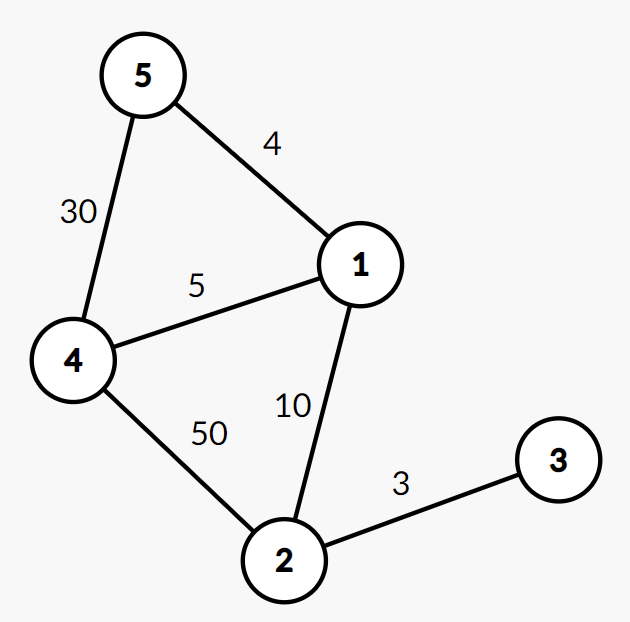
\includegraphics[height=6in]{mencari-tempat-perkumpulan.png}}

Dapat dibuktikan bahwa rumah nomor 1 merupakan rumah optimal untuk berkumpul:

\begin{center}
    \begin{itemize}
        \item $S_1$ = max(jarak rumah 3 ke rumah 1, jarak rumah 4 ke rumah 1, jarak rumah 5 ke rumah 1)
        \item $S_1$ = max(4, 5, 13)
        \item $S_1$ = 13
    \end{itemize}
\end{center}

Perhatikan bahwa bisa saja rumah berkumpul termasuk dari rumah nomor giant, suneo, atau nobita.
\end{document}